%%%%%%%%%%%%%%%%%%%%%%%%%%%%%%%%%%%%%%%%%%%%%%%%%%%%%%%%%%%%%%%%%%%%%%%%%%%%%%%%
\section{Experimental Setup}
\label{sec:experimental_setup}
% Setup of experiment (trying to prove anomaly is superset of risk indicators)
%%%%%%%%%%%%%%%%%%%%%%%%%%%%%%%%%%%%%%%%%%%%%%%%%%%%%%%%%%%%%%%%%%%%%%%%%%%%%%%%

%%%%%%%%%%%%%%%%%%%%%%%%%%%%%%%%%%%%%%%%
\subsection{Dataset}
\label{sec:experimental_setup_dataset}
% Which datasets did we use? (NGSIM - what about Motorway Turbulence?)
%%%%%%%%%%%%%%%%%%%%%%%%%%%%%%%%%%%%%%%%

We will train our model on the US Highway 101 (US-101) and Interstate 80 Freeway (I-80) data from the Next Generation Simulation (NGSIM) dataset \cite{colyar2007us,halkias2006ngsim}.
NGSIM is recorded at 10Hz, using stationary digital video cameras on top of tall buildings.
The distance between the camera and the highway, camera angle, and image quality result in the NGSIM dataset containing significant amounts of noise and other limitations \cite{punzo2011assessment,thiemann2008estimating}.
To minimize these effects, we use a Savitsky-Golay \cite{savitzky1964smoothing} filter to smooth vehicle positions over time, which in turn are used to recalculate each vehicles velocity and acceleration.

%%%%%%%%%%%%%%%%%%%%%%%%%%%%%%%%%%%%%%%%
\subsection{Interactions}
\label{sec:experimental_setup_interactions}
% Which interactions did we model? (Longitudinal)
%%%%%%%%%%%%%%%%%%%%%%%%%%%%%%%%%%%%%%%%

For our experiments we only focus on longitudinal vehicle interactions.
Therefore, we first extracted all same-lane longitudinal vehicle pairs (leader-follower).
Each vehicle pair which at any moment in time has an inter-vehicle-distance of less that 0 is dropped from further consideration (whist this would in theory indicate an accident has happened, in NGSIM this happens frequently due to data noise).
Interactions of interested between a leading ($l$) and following ($f$) vehicle are extracted from the data with a hysteresis loop:

\begin{equation}
\label{eqn:interaction_start}
\frac{\Delta X}{V_f} <= 2 \lor \Delta X <= 20
\end{equation}

\begin{equation}
\label{eqn:interaction_end}
\frac{\Delta X}{V_f} > 4 \land \Delta X > 40
\end{equation}

Equation \ref{eqn:interaction_start} defines the start of an interaction, and Equation \ref{eqn:interaction_end} the end of an interaction, where $\Delta X$ is the inter-vehicle-distance between both vehicles, and $V$ is a vehicles velocity.
Note that the first part of both equations ($\frac{\Delta X}{V_f}$) correspond to the Time Headway (THW) between both vehicles.

%%%%%%%%%%%%%%%%%%%%%%%%%%%%%%%%%%%%%%%%
\subsection{Autoencoder}
\label{sec:experimental_setup_autoencoder}
% Which Autoencoder structure/parameters/thresholds did we use?
%%%%%%%%%%%%%%%%%%%%%%%%%%%%%%%%%%%%%%%%

\begin{figure}
\includesvg[width=1.0\linewidth]{figs/autoencoder}
%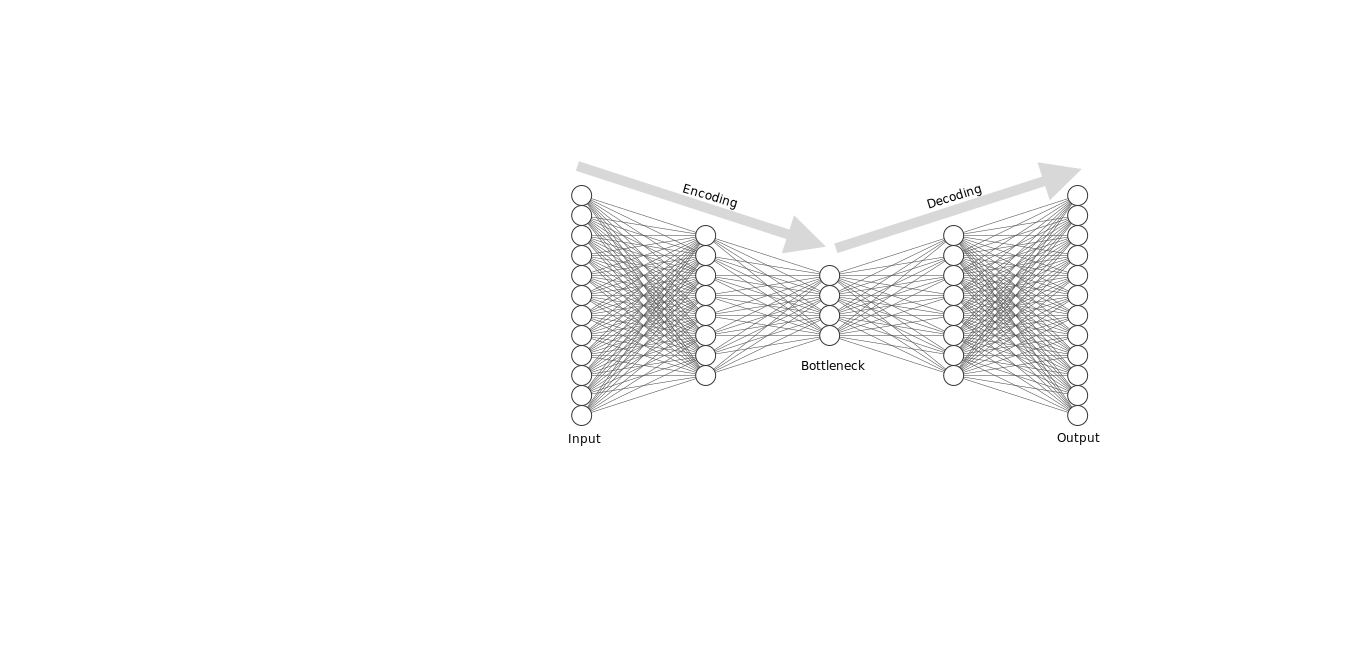
\includegraphics[]{figs/autoencoder}
\caption{A typical autoencoder architecture. Input values get encoded }
\label{fig:autoencoder}
\end{figure}

%%%%%%%%%%%%%%%%%%%%%%%%%%%%%%%%%%%%%%%%
\subsection{Risk Indicators}
\label{sec:experimental_setup_risk_indicators}
% Which risk indicators do we use to compare our results with?
%%%%%%%%%%%%%%%%%%%%%%%%%%%%%%%%%%%%%%%%